
\begin{frame}
  \maketitle
\end{frame}

\section{本編}
\begin{frame}{背景・目的}
  \begin{itemize}
  \item HPCにおけるネットワークのトポロジ(グラフ)
    \begin{itemize}
    \item 正則(すべてのスイッチは同一個数のポートを有する)
    \item 平均頂点間距離が短いと遅延も短い
      \cite{Koibuchi2012,Singla2011}
    \end{itemize}
  \item 平均頂点間距離が短い正則グラフを求める試み
    \cite{Fujita2015,Yamamoto2016,Fujiwara2015}
  \end{itemize}
  \begin{columns}[T]
    \begin{column}{.5\textwidth}
      \begin{itemize}
      \item \alert{一般化ムーアグラフ}
        \begin{itemize}
        \item 平均頂点間距離が理論的な下界に等しい正則グラフ
          \cite{Cerf1973,Cerf1974Lower}
        \item グラフの性質を利用した探索法は知られていない
        \end{itemize}
      \end{itemize}
    \end{column}
    \begin{column}{.5\textwidth}
      \begin{figure}
        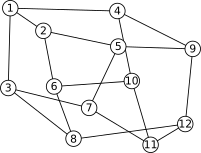
\includegraphics[width=.6\linewidth]{gmg-example}
        \caption{一般化ムーアグラフの例}
      \end{figure}
    \end{column}
  \end{columns}
  \begin{block}{}
    目的 : 一般化ムーアグラフの探索を効率的に行う方法の提案と評価
  \end{block}
\end{frame}

\begin{frame}[allowframebreaks]{探索アルゴリズム}
  \begin{columns}
    \begin{column}{.4\textwidth}
      \parbox[t]{\columnwidth}{
        \centering
        \includegraphics[width=.8\columnwidth]
                        {feasible-edges-example-color}
      }
    \end{column}
    \begin{column}{.6\textwidth}
      \begin{enumerate}
      \item 初期状態のグラフ(黒)から探索開始
      \item 逐次,候補辺(赤)を追加したグラフと
        追加しないグラフを生成し次に進む
      \item 定理\ref{thm:gmg-geom}を満たす可能性がないなら
        それ以降の探索を行わない
      \end{enumerate}
    \end{column}
  \end{columns}
  \begin{theorem}
    \label{thm:gmg-geom}
    正則グラフ$(n,k)$が一般化ムーアグラフであることの必要十分条件は
    次の二つの条件を同時に満たすことである.
    \begin{enumerate}
    \item 長さ$2Q$以下の閉路が存在しない
      \label{itm:gmg-geom-1}
    \item $R=0$なら直径が$Q$,\:$R>0$なら直径が$Q+1$
      \label{itm:gmg-geom-2}
    \end{enumerate}
    \[ Q=\max\{q|n-1-\sum_{i=1}^{q}k(k-1)^{i-1}\geq 0\},\:
    R=n-1-\sum_{i=1}^{Q}k(k-1)^{i-1} \]
  \end{theorem}
\end{frame}

\begin{frame}{探索空間の削減}
  \begin{columns}[T]
    \begin{column}{.5\textwidth}
      \begin{itemize}
        \item 初期グラフの変更
          \begin{itemize}
          \item 閉路を含むグラフ(閉路)
            \par\vbox{\parbox[t]{\columnwidth}{
                \centering
                \includegraphics[width=.7\columnwidth]
                                {initial-tree-cycle-example}
            }}
          \item 全域木
            \par\vbox{\parbox[t]{\columnwidth}{
                \centering
                \includegraphics[width=.7\columnwidth]
                                {initial-spanning-tree-12-example}
            }}
          \end{itemize}
      \end{itemize}
    \end{column}
    \begin{column}{.5\textwidth}
      \begin{itemize}
      \item 直径を考慮した枝刈り
        \par まだ見ていない辺をすべて追加したグラフの直径を計算
        \par 条件\ref{itm:gmg-geom-2}の直径より大きければ枝刈り
        \par\vbox{\parbox[t]{\columnwidth}{
          \centering
          \includegraphics[width=.9\columnwidth]{max-graph-example-color}
        }}
      \end{itemize}
    \end{column}
  \end{columns}
\end{frame}

\begin{frame}{実験}
  \begin{itemize}
  \item 測定項目
    \begin{enumerate}
    \item 探索時間(10回の平均を算出)
    \item 展開状態数
    \end{enumerate}
  \item パラメータ
    \begin{itemize}
    \item[]\par$\begin{aligned}
      k &= 3 \\
      n &= 4,6,8,10,12,14,16,18
    \end{aligned}$
    \end{itemize}
  \item 実行環境
    \par\begin{table}
    \scriptsize
    \caption{実行環境}
    \label{tab:env-lab}
    \centering
    \begin{tabular}{ll}
      \hline
      プロセッサ & Intel® Core™ i5-4670 CPU @ 3.40GHz × 4 \\ \hline
      メインメモリ & 5.8GiB \\ \hline
      ベースシステム & Ubuntu 16.04.3 LTS 64 ビット \\ \hline
      仮想化 & Oracle VirtualBox バージョン 5.1.18 \\ \hline
      ホストOS & Windows 8.1 Pro 64 ビット \\ \hline
      コンパイラ & gcc 5.4.0 \\ \hline
      グラフライブラリ & igraph 0.7.1-2.1 \\ \hline
      最適化フラグ & -Ofast \\ \hline
    \end{tabular}
    \end{table}
  \end{itemize}
\end{frame}

\begin{frame}{結果}
  \begin{columns}[T]
    \begin{column}{.5\textwidth}
      \begin{itemize}
      \item 全域木から探索を開始すれば最速かつ最も展開状態数が少ない
      \item 閉路は頂点数12で基本より展開状態数が多い
        \begin{itemize}
        \item 候補辺が適切な順番でなく,正則グラフになる可能性の判定が遅くなるため
        \end{itemize}
        \medskip
      \item 枝刈りによって展開状態数が減少し効率化に成功した
      \item 比較的小さい頂点数に対して探索時間が増加
        \begin{itemize}
        \item 必要なグラフが2個になり多くのグラフの生成と破棄が発生するため
        \end{itemize}
      \end{itemize}
    \end{column}
    \begin{column}{.5\textwidth}
      \centering
      \includegraphics[height=.35\textheight]{cmp-algo-time}
      \captionof{figure}{平均探索時間}
      \vfill
      \includegraphics[height=.35\textheight]{cmp-algo-state}
      \captionof{figure}{グラフ取り出し回数}
    \end{column}
  \end{columns}
\end{frame}

\begin{frame}{まとめ}
  \begin{itemize}
  \item 一般化ムーアグラフの探索の探索空間の削減の効果を研究
    \begin{itemize}
    \item 全域木から探索を始める
    \item 直径を考慮した枝刈りを採用する
    \end{itemize}
  \item[] 効率が良く最速で探索できる
  \item 今後の課題
    \begin{itemize}
    \item 提案した初期状態から探索を開始することの妥当性の証明
    \item 一般化ムーアグラフが存在しないときの平均頂点間距離最小のグラフ
    \end{itemize}
  \end{itemize}
  \begin{figure}
    \centering
    \includegraphics[width=\textwidth]{gmg-existence-h}
    \caption{発見した一般化ムーアグラフの頂点数と次数の組}
  \end{figure}
\end{frame}

\appendix
%\begin{frame}<handout:0>{付録}
%  ふろくです
%\end{frame}

\begin{frame}[allowframebreaks]{参考文献}
  \bibliography{../res/MyCollection}
\end{frame}


